%%%%%%%%%%%%%%%%%%%%%%%%%%%%%%%%%%%
%This is the LaTeX ARTICLE template for RSC journals
%Copyright The Royal Society of Chemistry 2016
%%%%%%%%%%%%%%%%%%%%%%%%%%%%%%%%%%%

\documentclass[twoside,twocolumn,9pt]{article}
\usepackage{extsizes}
\usepackage[super,sort&compress,comma]{natbib} 
\usepackage[version=3]{mhchem}
\usepackage[left=1.5cm, right=1.5cm, top=1.785cm, bottom=2.0cm]{geometry}
\usepackage{balance}
\usepackage{mathptmx}
\usepackage{sectsty}
\usepackage{graphicx} 
\usepackage{lastpage}
\usepackage[format=plain,justification=justified,singlelinecheck=false,font={stretch=1.125,small,sf},labelfont=bf,labelsep=space]{caption}
\usepackage{float}
\usepackage{fancyhdr}
\usepackage{fnpos}
\usepackage[english]{babel}
\addto{\captionsenglish}{%
  \renewcommand{\refname}{Notes and references}
}
\usepackage{array}
\usepackage{droidsans}
\usepackage{charter}
\usepackage[T1]{fontenc}
\usepackage[usenames,dvipsnames]{xcolor}
\usepackage{setspace}
\usepackage[compact]{titlesec}
\usepackage{hyperref}
%%%Please don't disable any packages in the preamble, as this may cause the template to display incorrectly.%%%


\usepackage{epstopdf}%This line makes .eps figures into .pdf - please comment out if not required.

\definecolor{cream}{RGB}{222,217,201}

%%%%%%%%% Preamble of the bibliography, can be commented or deleted 
%%\def\bibpreamble{For the reference section, the style file \texttt{rsc.bst} can be used to generate the correct reference style.\footnotemark[4]
%%\begin{enumerate}
%%\item{Citations should appear here in the format A. Name, B. Name and C. Name, \emph{Journal Title}, 2000, \textbf{35}, 3523;} 
%%\item{A. Name, B. Name and C. Name, \emph{Journal Title, 2000}, \textbf{35}, 3523.}
%%\end{enumerate}
%%... \\\\
%%We encourage the citation of primary research over review articles, where appropriate, in order to give credit to those who first reported a finding. \href{https://www.rsc.org/news-events/articles/2020/jun/rsc-signs-dora/}{Find out more about our commitments to the principles of San Francisco Declaration on Research Assessment (DORA).}}
%%%%%%%%% 

\begin{document}

\pagestyle{fancy}
\thispagestyle{plain}
\fancypagestyle{plain}{
%%%HEADER%%%
\renewcommand{\headrulewidth}{0pt}
}
%%%END OF HEADER%%%

%%%PAGE SETUP - Please do not change any commands within this section%%%
\makeFNbottom
\makeatletter
\renewcommand\LARGE{\@setfontsize\LARGE{15pt}{17}}
\renewcommand\Large{\@setfontsize\Large{12pt}{14}}
\renewcommand\large{\@setfontsize\large{10pt}{12}}
\renewcommand\footnotesize{\@setfontsize\footnotesize{7pt}{10}}
\makeatother

\renewcommand{\thefootnote}{\fnsymbol{footnote}}
\renewcommand\footnoterule{\vspace*{1pt}% 
\color{cream}\hrule width 3.5in height 0.4pt \color{black}\vspace*{5pt}} 
\setcounter{secnumdepth}{5}

\makeatletter 
\renewcommand\@biblabel[1]{#1}            
\renewcommand\@makefntext[1]% 
{\noindent\makebox[0pt][r]{\@thefnmark\,}#1}
\makeatother 
\renewcommand{\figurename}{\small{Fig.}~}
\sectionfont{\sffamily\Large}
\subsectionfont{\normalsize}
\subsubsectionfont{\bf}
\setstretch{1.125} %In particular, please do not alter this line.
\setlength{\skip\footins}{0.8cm}
\setlength{\footnotesep}{0.25cm}
\setlength{\jot}{10pt}
\titlespacing*{\section}{0pt}{4pt}{4pt}
\titlespacing*{\subsection}{0pt}{15pt}{1pt}
%%%END OF PAGE SETUP%%%

%%%FOOTER%%%
\fancyfoot{}
\fancyfoot[LO,RE]{\vspace{-7.1pt}
\includegraphics[height=9pt]{head_foot/LF}}
\fancyfoot[CO]{\vspace{-7.1pt}\hspace{13.2cm}
\includegraphics{head_foot/RF}}
\fancyfoot[CE]{\vspace{-7.2pt}\hspace{-14.2cm}
\includegraphics{head_foot/RF}}
\fancyfoot[RO]{\footnotesize{\sffamily{1--\pageref{LastPage} ~\textbar  \hspace{2pt}\thepage}}}
\fancyfoot[LE]{\footnotesize{\sffamily{\thepage~\textbar\hspace{3.45cm} 1--\pageref{LastPage}}}}
\fancyhead{}
\renewcommand{\headrulewidth}{0pt} 
\renewcommand{\footrulewidth}{0pt}
\setlength{\arrayrulewidth}{1pt}
\setlength{\columnsep}{6.5mm}
\setlength\bibsep{1pt}
%%%END OF FOOTER%%%

%%%FIGURE SETUP - please do not change any commands within this section%%%
\makeatletter 
\newlength{\figrulesep} 
\setlength{\figrulesep}{0.5\textfloatsep} 

\newcommand{\topfigrule}{\vspace*{-1pt}% 
\noindent{\color{cream}\rule[-\figrulesep]{\columnwidth}{1.5pt}} }

\newcommand{\botfigrule}{\vspace*{-2pt}% 
\noindent{\color{cream}\rule[\figrulesep]{\columnwidth}{1.5pt}} }

\newcommand{\dblfigrule}{\vspace*{-1pt}% 
\noindent{\color{cream}\rule[-\figrulesep]{\textwidth}{1.5pt}} }

\makeatother
%%%END OF FIGURE SETUP%%%

%%%TITLE, AUTHORS AND ABSTRACT%%%
\twocolumn[
  \begin{@twocolumnfalse}
{
\includegraphics[height=30pt]{head_foot/journal_name}\hfill\raisebox{0pt}[0pt][0pt]{
\includegraphics[height=55pt]{head_foot/RSC_LOGO_CMYK}}\\[1ex]

\includegraphics[width=18.5cm]{head_foot/header_bar}}\par
\vspace{1em}
\sffamily
\begin{tabular}{m{4.5cm} p{13.5cm} }


\includegraphics{head_foot/DOI} & \noindent\LARGE{\textbf{Adaptive Distribution-Driven Filtering in Reinforcement Learning applied to GLP-1R Modulator Design}} \\%Article title goes here instead of the text "This is the title"
\vspace{0.3cm} & \vspace{0.3cm} \\

 & \noindent\large{Joan Clark-Nicolas,\textit{$^{*,a,1}$} Angelo Pugliese,\textit{$^{b}$} and Angus Morrison\textit{$^{b}$}} \\

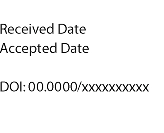
\includegraphics{head_foot/dates} & \noindent\normalsize{The vastness of theoretical drug-like chemical space presents a fundamental challenge for modern drug discovery. Here, we present a generative workflow that addresses this issue through the integration of reinforcement learning-driven molecular generation, adaptive distribution-driven filtering, and transfer learning. The workflow leverages the REINVENT framework and employs adaptive selection criteria based on iteration-specific histogram peaks to avoid reliance on fixed thresholds. Structure-based evaluation is performed using ensemble docking into multiple receptor conformations derived from molecular dynamics simulations, combined with protein-ligand contact surface area (CSA) calculations. As a test case, we applied this approach to the design of novel positive allosteric modulators (PAMs) of the glucagon-like peptide-1 receptor (GLP-1R) acting via a "molecular glue" mechanism to stabilize the endogenous agonist-receptor interface. Across iterations, the workflow yielded consistent enrichment in predicted binding affinity, drug-likeness, and synthetic accessibility. Notably, the top-ranking candidates significantly outperformed the reference compound in docking scores and drug-likeness while successfully recapitulating the glue-like interaction profile. These results demonstrate the ability of the proposed closed-loop framework to steer generative models toward target-relevant regions of chemical space and generate diverse, high-quality candidate molecules.} \\%The abstrast goes here instead of the text "The abstract should be..."

\end{tabular}

 \end{@twocolumnfalse} \vspace{0.6cm}

  ]
%%%END OF TITLE, AUTHORS AND ABSTRACT%%%

%%%FONT SETUP - please do not change any commands within this section
\renewcommand*\rmdefault{bch}\normalfont\upshape
\rmfamily
\section*{}
\vspace{-1cm}


%%%FOOTNOTES%%%
\footnotetext{\textit{$^{a}$~} University of Lincoln, Brayford Pool, Lincoln, Lincolonshire, LN6 7TS, England, United Kingdom}
\footnotetext{\textit{$^{1}$~} Current affiliation: WestCHEM, Department of Pure and Applied Chemistry, University of Strathclyde, 204 George St, Glasgow, Lanarkshire, G1 1XW, Scotland, United Kingdom}
\footnotetext{\textit{$^{b}$~} BioAscent Discovery Ltd, Bo’Ness Road, Newhouse, Lanarkshire, ML1 5UH, Scotland, United Kingdom}
\footnotetext{\textit{*} Corresponding Author: joan.clark-nicolas@strath.ac.uk}

%Please use \dag to cite the ESI in the main text of the article.
%If you article does not have ESI please remove the the \dag symbol from the title and the footnotetext below.
%\footnotetext{\dag~Supplementary Information available: [details of any supplementary information available should be included here]. See DOI: 00.0000/00000000.}
%additional addresses can be cited as above using the lower-case letters, c, d, e... If all authors are from the same address, no letter is required

%%\footnotetext{\dag~Additional footnotes to the title and authors can be included \textit{e.g.}\ `Present address:' or `These authors contributed equally to this work' as above using the symbols: \ddag, \textsection, and \P. Please place the appropriate symbol next to the author's name and include a \texttt{\textbackslash footnotetext} entry in the the correct place in the list.}


%%%END OF FOOTNOTES%%%

%%%MAIN TEXT%%%%
\section{Introduction}
Estimates suggest that the number of realistic drug-like molecules could be as high as $10^{60}$, far exceeding the size of even the largest enumerated databases and available screening libraries, rendering exhaustive enumeration infeasible and necessitating intelligent sampling strategies\cite{Bohacek1996ThePerspective,Polishchuk2013EstimationData,Walters2019VirtualLibraries}. This combinatorial enormity highlights the need for computational methods capable of effectively exploring and exploiting relevant areas of chemical space in search of biologically active compounds.

Generative artificial intelligence (GenAI) has emerged as a promising paradigm for addressing aspects of this challenge by enabling data-driven de novo molecular design. The past decade has seen the emergence of a wide range of generative modeling approaches, including variational autoencoders (VAEs)\cite{Gomez-Bombarelli2018AutomaticMolecules,Oliveira2022MolecularAutoencoder,Ochiai2023VariationalComplexity},
generative adversarial networks (GANs)\cite{Lee2021GenerativeDesign,Macedo2024MedGAN:Design,Sun2025GenerativeChallenges,Xu2025GenerationNetworks},
autoregressive models\cite{Segler2017GeneratingNetworks,Gebauer2022InverseNetworks} and  
diffusion models\cite{Morehead2024Geometry-completeOptimization}. These approaches aim to learn implicit representations of chemical space from existing molecular datasets and to generate novel compounds biased toward desirable physicochemical or biological properties.

A survey by Tang \textit{et al.} reviews those and other architectures in depth.
\cite{Tang2024AGeneration}. Among these methods, reinforcement learning (RL) has proven particularly attractive for drug discovery applications because it allows molecular generation to be formulated as a sequential decision-making process guided by explicit reward functions. In this setting, molecular structures are iteratively modified to maximize one or more objectives, such as predicted binding affinity, physicochemical property ranges, or synthetic accessibility. Early RL-based frameworks demonstrated the feasibility of directly optimizing molecular properties \textit{in silico}, but were often limited by instability, mode collapse, or lack of chemical diversity\cite{Walters2020AssessingChemistry}. Subsequent developments introduced more robust architectures, improved molecular representations, and better reward shaping strategies—such as policy-gradient optimization over pretrained generative models, graph-based action spaces, and multi-objective reward formulations—significantly improving the practical utility of RL-driven molecular design\cite{Olivecrona2017MolecularLearning,Zhou2019OptimizationLearning,Blaschke2020Memory-assistedDesign}.

In parallel, transfer learning has become a central component of modern generative chemistry workflows\cite{Segler2017GeneratingNetworks,Gomez-Bombarelli2018AutomaticMolecules}. Models pretrained on large, chemically diverse datasets can be fine-tuned on smaller, task-specific datasets, enabling more efficient learning when data for a particular target or property are scarce. This approach has been shown to improve sample efficiency and reduce overfitting, particularly in early-stage discovery contexts where only limited bioactivity data are available. Contemporary generative frameworks such as REINVENT explicitly integrate transfer learning with reinforcement learning to enable iterative optimization of molecular libraries towards complex, multi-parameter objectives\cite{Blaschke2020ReinventDesign,Loeffler2024ReinventDesign}.

Despite these advances, the application of generative AI to real-world drug discovery remains constrained by several fundamental limitations. One of the most significant challenges is data scarcity, especially for novel or underexplored biological targets. Although large public repositories such as ChEMBL contain extensive activity data for well-studied targets, many therapeutically relevant proteins are associated with only a small number of known ligands. In such low-data regimes, both generative models and the predictive models used to evaluate generated compounds can exhibit poor generalization, leading to chemically unrealistic designs or over-exploitation of a narrow set of known scaffolds\cite{Walters2020AssessingChemistry,Tang2024AGeneration}.

Closely related to data scarcity is the issue of chemical bias. Generative models trained on existing datasets tend to reproduce patterns present in the training data, which can limit their ability to propose genuinely novel chemotypes. This bias is particularly problematic when innovation beyond known chemical matter is required, for example when targeting allosteric sites or protein classes with limited precedent. Even when novelty metrics are explicitly incorporated into reward functions, achieving a balance between novelty, validity, and target relevance remains a non-trivial challenge.

Another important limitation concerns synthetic feasibility. Many generative models optimize abstract molecular descriptors without explicitly considering whether proposed compounds can be synthesized using realistic chemical routes. As a result, a substantial fraction of generated molecules may be impractical for experimental follow-up. While post-hoc filtering using synthetic accessibility scores or retrosynthetic analysis can mitigate this issue, tighter integration of synthetic constraints into the generative process itself remains an active area of research\cite{Tang2024AGeneration}.

Furthermore, the rapid pace at which generative models can propose new molecules often outstrips the capacity of downstream evaluation pipelines. High-quality assessment of generated compounds—whether via structure-based docking, molecular dynamics simulations, or experimental assays—remains computationally and experimentally expensive. This imbalance can limit the effective feedback available to generative models and slow iterative optimization cycles, particularly in resource-constrained discovery programs.

To address some of these challenges, hybrid workflows that combine generative AI with physics-based or structure-based evaluation methods have gained increasing attention. By integrating virtual screening, geometric or pharmacophoric descriptors, and iterative retraining, such workflows aim to ground generative exploration in biologically meaningful feedback while maintaining flexibility in chemical design space. Reinforcement learning frameworks are particularly well suited to this setting, as they naturally accommodate iterative reward updates based on increasingly informative evaluation criteria. In this work, we propose an iterative workflow that leverages the reinforcement learning and transfer learning capabilities of REINVENT4 and combines them with virtual screening and geometric descriptor calculation to progressively bias molecular generation toward compounds with desirable properties. This closed-loop strategy is designed to improve performance in low-data settings while maintaining chemical diversity and relevance.

As a test case, we apply this workflow to the design of novel positive allosteric modulators (PAMs) of the glucagon-like peptide-1 receptor (GLP-1R). GLP-1R is a class B G protein-coupled receptor that plays a central role in glucose homeostasis and is a clinically validated target for the treatment of type 2 diabetes\cite{Perfetti2000Glucagon-likeFunction}. While peptide-based GLP-1R agonists have achieved substantial clinical success, the discovery of small-molecule modulators has proven challenging. Positive allosteric modulation represents a particularly attractive strategy, as PAMs can enhance the activity of endogenous agonists without directly activating the receptor, potentially offering improved selectivity and safety profiles. Several small-molecule GLP-1R PAMs have been reported, and are analysed in depth in a review by Zhang \textit{et al.}\cite{Zhang2024BindingAgonists}. However, their limited potency and suboptimal physicochemical properties underscore the difficulty of identifying suitable chemical matter for this target\cite{Wang2021AllostericSite}. These characteristics make GLP-1R PAM discovery a stringent and relevant test case for evaluating generative AI workflows designed to operate under data-limited and chemically challenging conditions.

\section{Methods}
The overall objective of this workflow is to increase the availability of theoretical molecules with a desired set of predicted physical properties and binding affinity for the target of interest. To achieve this, we implemented an iterative generative–filtering–retraining strategy, illustrated in Figure \ref{fig:workflow}, that integrates molecular generation guided by Reinforcement Learning (RL), two filters based on physicochemical and structural properties, and model refinement via Transfer Learning (TL). This closed-loop process yields progressively refined molecular libraries tailored to target-specific design objectives.

\begin{figure}[H]
 \centering
 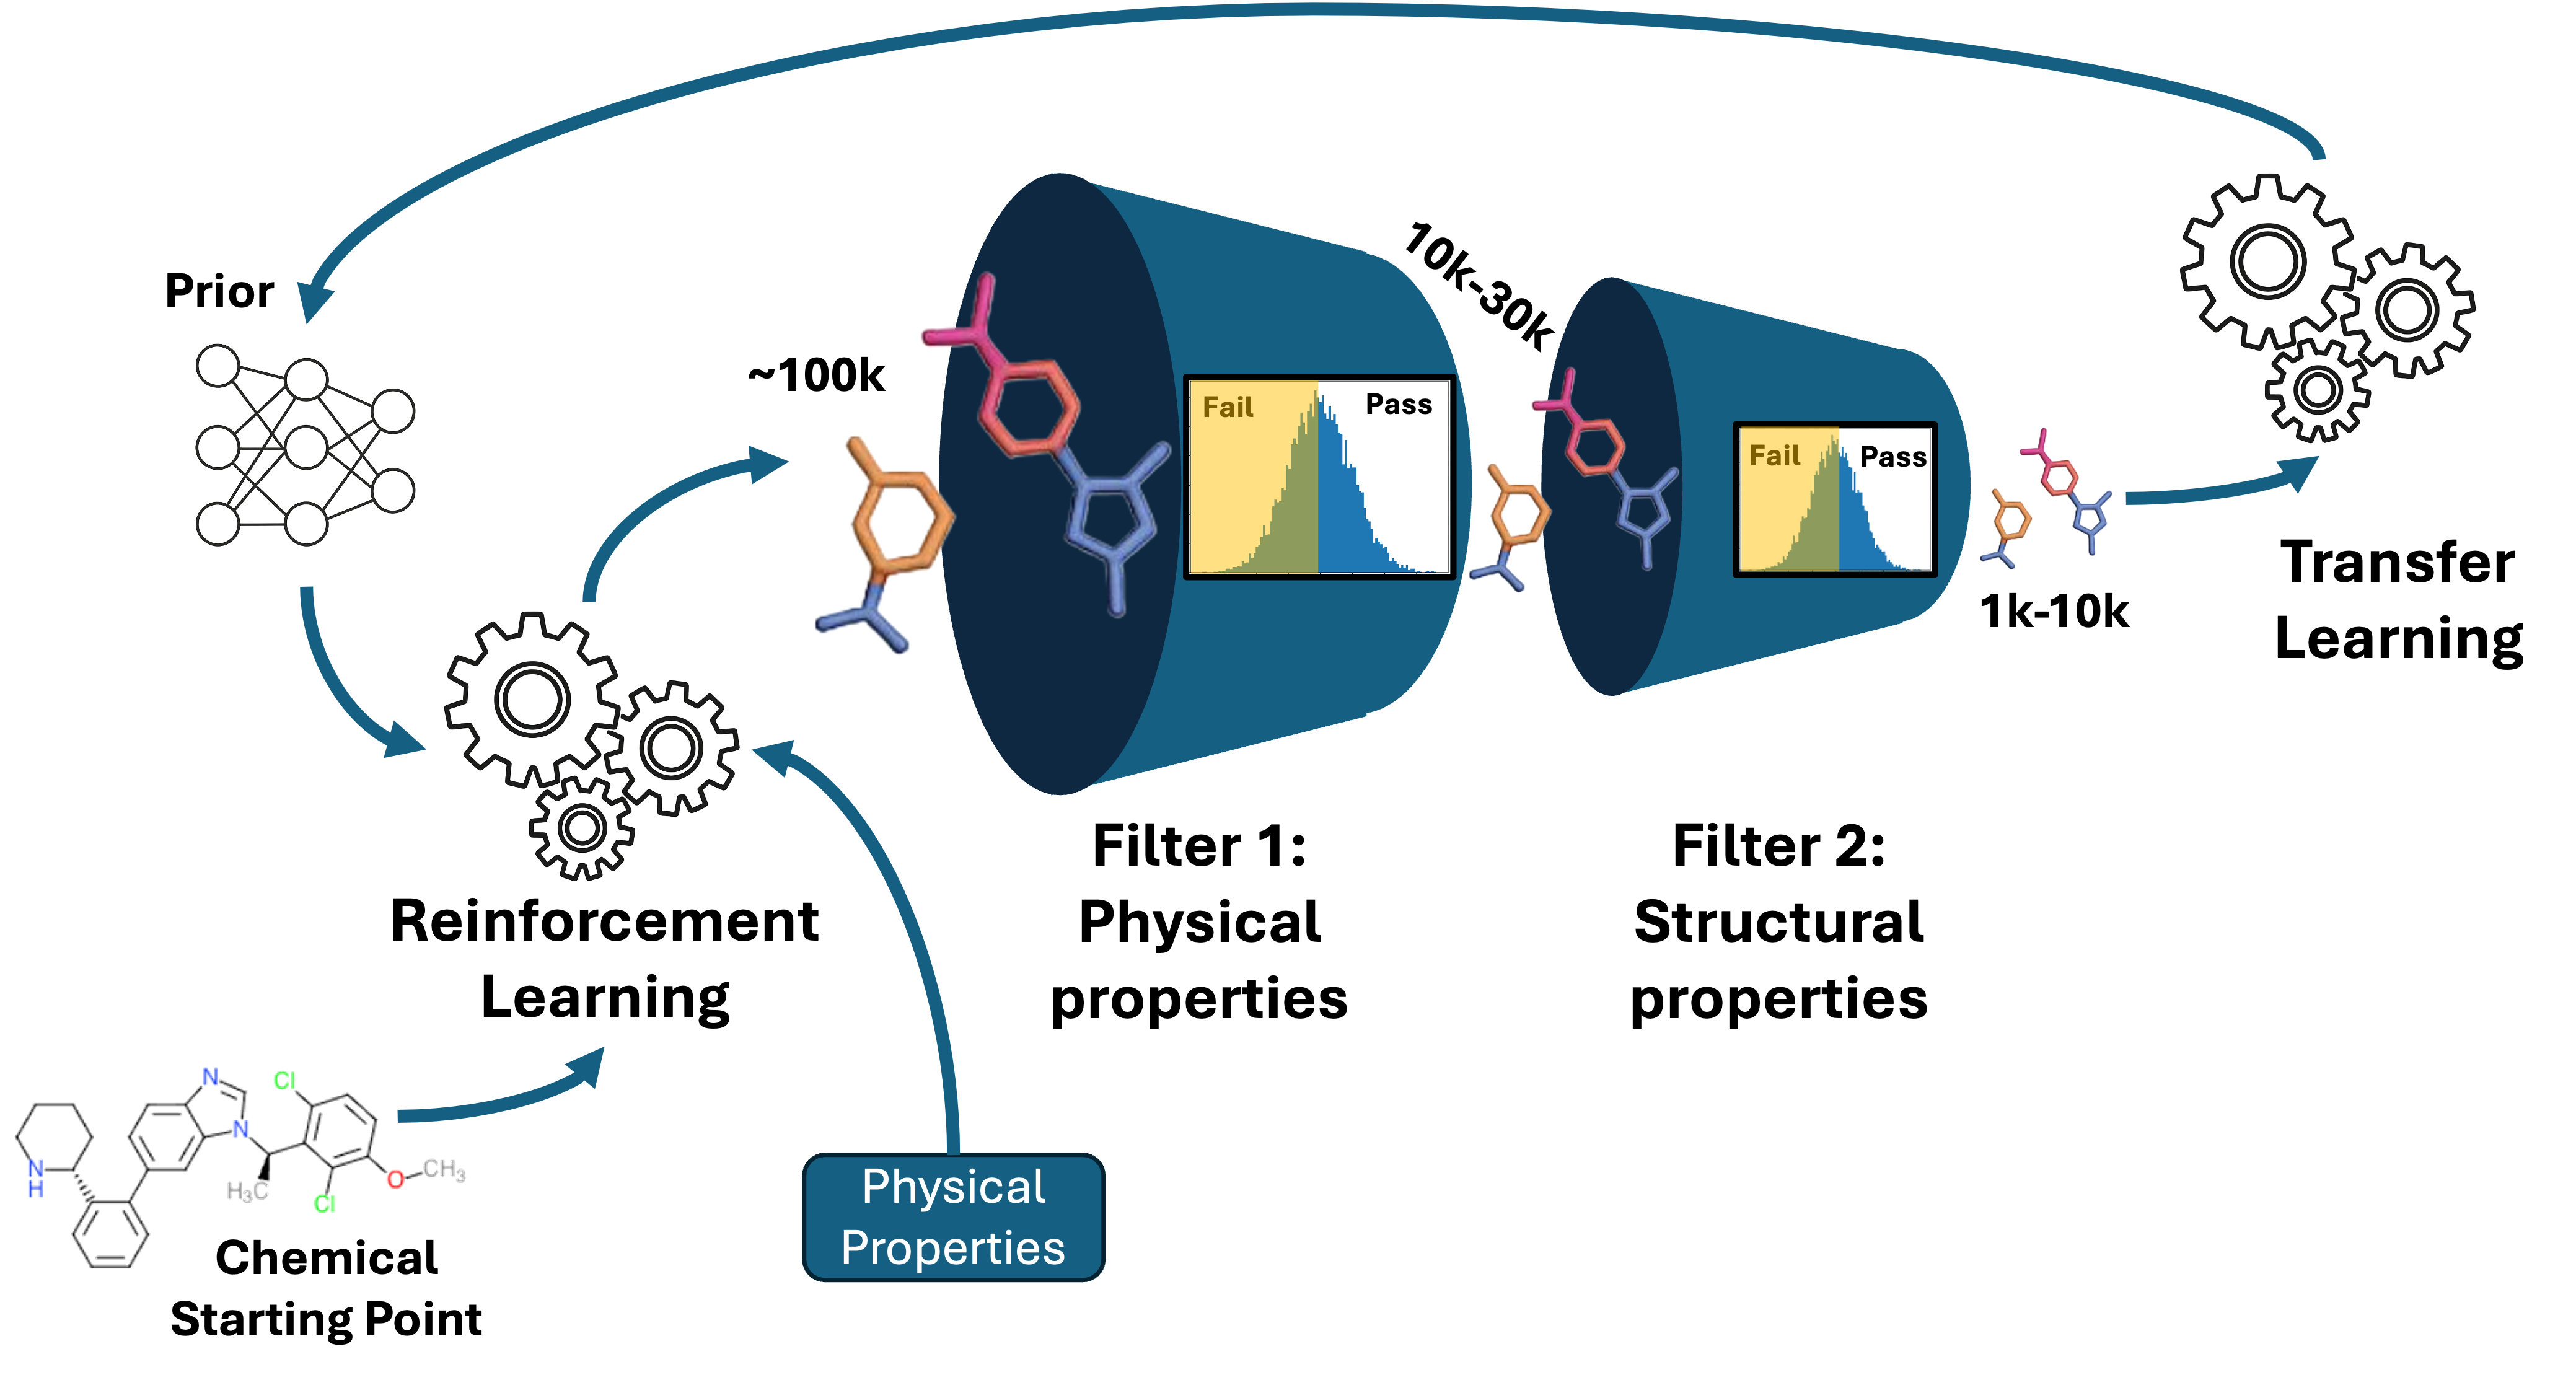
\includegraphics[width=\textwidth]{Figures/Workflow.png}
 \caption{Illustration of the proposed workflow. Beginning with a prior model, a set of target physicochemical properties, and optionally an initial SMILES seed, a reinforcement learning step generates roughly 100k candidate molecules. The distributions of predicted properties and negative log-likelihood are examined, and only molecules scoring better than the histogram peak for each property (typically 10–30k) are advanced. These compounds are then docked into 10 representative target structures, and contact surface area is computed for the top-ranked pose. A second filter is applied using the mean top docking score and mean contact surface area, yielding a refined set of approximately 1–10k molecules. This subset is subsequently used to retrain the prior, producing an updated model that is increasingly focused on the desired predicted binding affinity and physicochemical characteristics for the next iteration.}
 \label{fig:workflow}
\end{figure}

\subsection{Generating-Filtering-Refining Loop}\label{aloop}
In each cycle, a generative model with Reinforcement Learning (RL) capabilities is used to propose novel molecule datasets enriched for predefined physicochemical attributes. The resulting candidates are subsequently evaluated using two complementary filtering stages. In the first stage, we take into account the values of the predicted target properties and the negative-log likelihood (NLL), an estimation of how likely the model is to suggest a given item, of each of the generated molecules. The distributions of these quantities are then examined, and only molecules that score better than the histogram peak across all properties progress to the next filter. In the second stage, a structure-based filter incorporates docking scores and predicted protein–ligand contact surface area to approximate binding affinity and interaction quality.  Molecules that pass through both filters are then leveraged to update the generative prior using Transfer Learning (TL), thereby biasing future iterations toward regions of chemical space that are associated with the desired set of properties. 

\subsubsection{Model, Descriptors and Reinforcement Learning}
Molecular generation was performed using the REINVENT framework, which employs a recurrent neural network trained to model the probability distribution of valid SMILES sequences\cite{Blaschke2020ReinventDesign,Loeffler2024OptimalSimulations}. Although REINVENT was selected for its mature implementation of Reinforcement Learning and Transfer Learning for molecular design, the overall workflow is model-agnostic in principle and could be implemented using alternative generative architectures with comparable capabilities. At each iteration, the model consists of a prior and an agent network. Unlike conventional RL setups in which the prior remains fixed, both the prior and the agent were updated iteratively in this work. The publicly available REINVENT prior\cite{LofflerREINVENT4Priors} was used for the first iteration of the cycle. Subsequently, the model obtained after Transfer Learning at a given iteration served as both the prior and the agent initialization for the next. This closes the active learning loop and allows information gained from downstream filtering and docking to be propagated into subsequent generations. 

Three primary ligand-based descriptors were used during RL and subsequent filtering. First, the quantitative estimate of drug-likeness (QED)\cite{Wildman1999PredictionContributions,Bickerton2012QuantifyingDrugs} was used to guide the model towards molecules that would be predicted to have good oral bio-availability. Second, a synthetic accessibility score (SA score) was used to generate molecules likely to have a feasible synthetic route\cite{Ertl2009EstimationContributions}. Third the chemical dissimilarity (Tanimoto distance) to a reference SMILES sequence was used in order to generate molecules that increasingly differed from the chemical starting point described in Section \ref{section:chemical_starting_point}. All three descriptors were calculated using RDKit\cite{RDKit:Chemoinformatics} via the wrapper implemented in REINVENT4. Sigmoid functions were employed to map these descriptors onto a normalized scale from 0 to 1, where 0 denotes a molecule that does not exhibit the desired property and 1 denotes a molecule that fully satisfies it. The original ranges of those descriptors and the type of sigmoid used in each case are presented in table \ref{tab:rl_descriptors}. For this proof-of-concept, all descriptors were given a weight of 1, making them equally relevant in the RL scoring function and allowing simultaneous optimization of drug-likeness, synthetic accessibility, and chemical novelty relative to the reference compound.

\begin{table}[H]
  \caption{Functions used to normalise descriptors}
  \label{tab:rl_descriptors}
  \centering
  \begin{tabular}{ccc}
    \hline
    Descriptor & Original scale & Sigmoid\\
               & [worst,best]   &        \\
    \hline
    QED & [0-1] & Direct \\
    SA Score & [10-1] & Reverse \\
    Tanimoto Distance & [0-1] & Direct \\
    \hline
  \end{tabular}
\end{table}

1000 RL steps were run at each iteration. To prevent mode collapse and encourage structural diversity, a diversity filter based on Murcko scaffolds was applied during RL. Generated molecules sharing identical scaffolds were grouped into buckets, and a penalty was applied once a bucket exceeded a predefined size. This mechanism ensured continued exploration of chemical space while optimizing the scoring objective. The output of the RL stage at each iteration consisted of a population of newly generated SMILES sequences, along with the associated NLL and raw descriptor values. 

\subsubsection{First Filter}
The first filtering stage aimed to select molecules that were not only favored by the RL scoring function, but also statistically enriched relative to the bulk of the generated population. At each iteration, a histogram of each of the selected physico-chemical properties was constructed using only the molecules from the current iteration. For each histogram, the peak was defined as the center of the bin containing the largest number of molecules. These peak values served as adaptive, iteration-specific thresholds reflecting the desired characteristics of the generated population. A molecule would only be progressed to the next filter if it satisfied all the following criteria simultaneously:
\begin{itemize}
    \item Its associated NLL should be higher than that of the corresponding histogram peak, indicating a SMILES sequence that would be less probable under the current model.
    \item Its Tanimoto Distance value should be higher than the histogram peak, favouring an increased dissimilarity from the the chemical starting point.
    \item Its QED value should be higher than the histogram peak, indicating  a molecule likely to have higher oral bioavailability.
    \item Its SA score should be lower than the histogram peak, indicating a molecule more likely to be easily synthesizable.
\end{itemize}

The selection of molecules with a Negative Log-Likelihood (NLL) higher than the histogram peak is a deliberate strategy to prioritize 'model exploration' over 'exploitation.' By targeting SMILES sequences that are statistically less probable under the current model, we steer the generative process toward the 'edges' of the chemical space known by the model, thereby increasing the likelihood of identifying novel chemotypes rather than reinforcing existing biases. The conjunctive application of these criteria ensured that only molecules exhibiting favorable trends across all descriptors were advanced to the next filter. This distribution-based filtering strategy adapts automatically to changes in the generated chemical space across iterations and avoids reliance on fixed cutoffs.

\subsubsection{Second Filter}\label{section:second_filter}
Molecules that passed through the first filter were subjected to ensemble virtual screening and calculation of contact surface area between them and the relevant residues in the binding site. 
Three-dimensional, docking-ready ligand structures were generated using Meeko\cite{Santos-Martins2025Meeko:Beyond}, then VinaGPU-2.1\cite{Ding2023Vina-GPUUnits,Tang2024Vina-GPUDerivatives} was used to dock them into 10 different conformations of the receptor's binding site generated by Molecular Dynamics (MD) simulations. The selection of receptor structures for docking is discussed in the Results section. The resulting overall docking score of each ligand was defined as the geometric mean of the scores corresponding to the top-ranking pose obtained for each receptor structure.

The Contact Surface Area (CSA) between the GLP-1R/GLP-1 system and each ligand was calculated using the Shrake–Rupley solvent-accessible surface area (SASA) algorithm as implemented in MDTraj\cite{McGibbon2015MDTraj:Trajectories}. Specifically, for each top-ranking docking pose, the SASA was calculated separately for the isolated ligand, the isolated binding site, and the protein–ligand complex, then the contact surface area was then obtained using Equation \ref{eq:CSA}. The overall CSA of a given ligand was then expressed as the geometric mean of the CSA values obtained for the top ranking pose corresponding to docking that ligand on each of the selected MD snapshots.

\begin{equation}
\label{eq:CSA}
    CSA = SASA_{ligand}+SASA_{receptor}-SASA_{complex}
\end{equation}

Histograms of the overall docking scores and CSA values were constructed for the molecules entering the second filter at each iteration. As in the first filter, peak values were defined as the centers of the most populated bins. Molecules were retained if they simultaneously satisfied the two following criteria:
\begin{itemize}
\item An average docking score lower (more favourable) than the peak of the histogram.
\item An average CSA higher than the peak of the histogram.
\end{itemize}
This second filtering stage selected compounds that combined high predicted binding affinity and extensive physical contact between the ligands and the relevant residues in the binding site. 

The current docking-CSA approach provides an approximation to binding affinity that illustrates the ability of this workflow to iteratively improve the quality of the generated moelcules, but it does not explicitly account for water-mediated hydrogen bonds. Given the hypothesized role of Lys202 in the GLP-1R PAM binding site, the inclusion of explicit-water docking protocols or hydrated interaction descriptors in future iterations may further refine the selection of high-potency candidates.

\subsubsection{Model Refinement via Transfer Learning}
Molecules that passed both filtering stages were used to refine the generative model via transfer learning. The selected compounds were randomly split into a training set (75\%) and a validation set (25\%). No independent test set was defined, as the objective of this step was model adaptation, rather than performance benchmarking. At each iteration, transfer learning was initialized from the model obtained at the end of the RL stage of the same iteration. The model was fine-tuned to increase the likelihood of the filtered molecules, biasing subsequent generations toward chemical features associated with favorable properties.

The resulting fine-tuned model served as the starting point for the next iteration of the active learning loop, functioning as both prior and agent for the RL step. This RL–filtering–TL cycle was repeated for five iterations. Although the number of iterations was limited by practical considerations, the observed progression was sufficient to demonstrate that the workflow systematically enriches generated compounds toward the targeted physicochemical and binding-related properties.

\subsection{Selection of a chemical starting point}\label{section:chemical_starting_point}
Where one or more chemical starting points are available, they can be included in the workflow in order to generate molecules that differ from them in terms of chemical similarity as well as outperforming them in terms of predicted binding affinity and chemical properties. The chosen chemical starting point for this proof-of-concept was Compound LSN3160440, a GLP-1R PAM originally reported by Bueno \textit{et al}\cite{Bueno2020StructuralReceptor}. As depicted in Figure \ref{fig:lsn-interactions}, LSN3160440 binds in a pocket located between helices TM1 and TM2 of GLP-1R, forming $\pi-\pi$ stacking interactions with residue Tyr145 at TM1 and van der Waals interactions with residues Leu142 at TM1, and Phe12, Val16 and Leu20 from GLP-1. The original publication also hypothesized a water-mediated hydrogen bond between LSN3160440 and Lys202 at TM2, which the authors also observed in MD simulations. This interaction pattern suggests that LSN3160440 acts a molecular glue that enhances the interactions between GLP-1R and its natural substrate GLP-1, as opposed to more traditional GLP-1R agonists, which bind the receptor competitively.

\begin{figure}[H]
\centering
  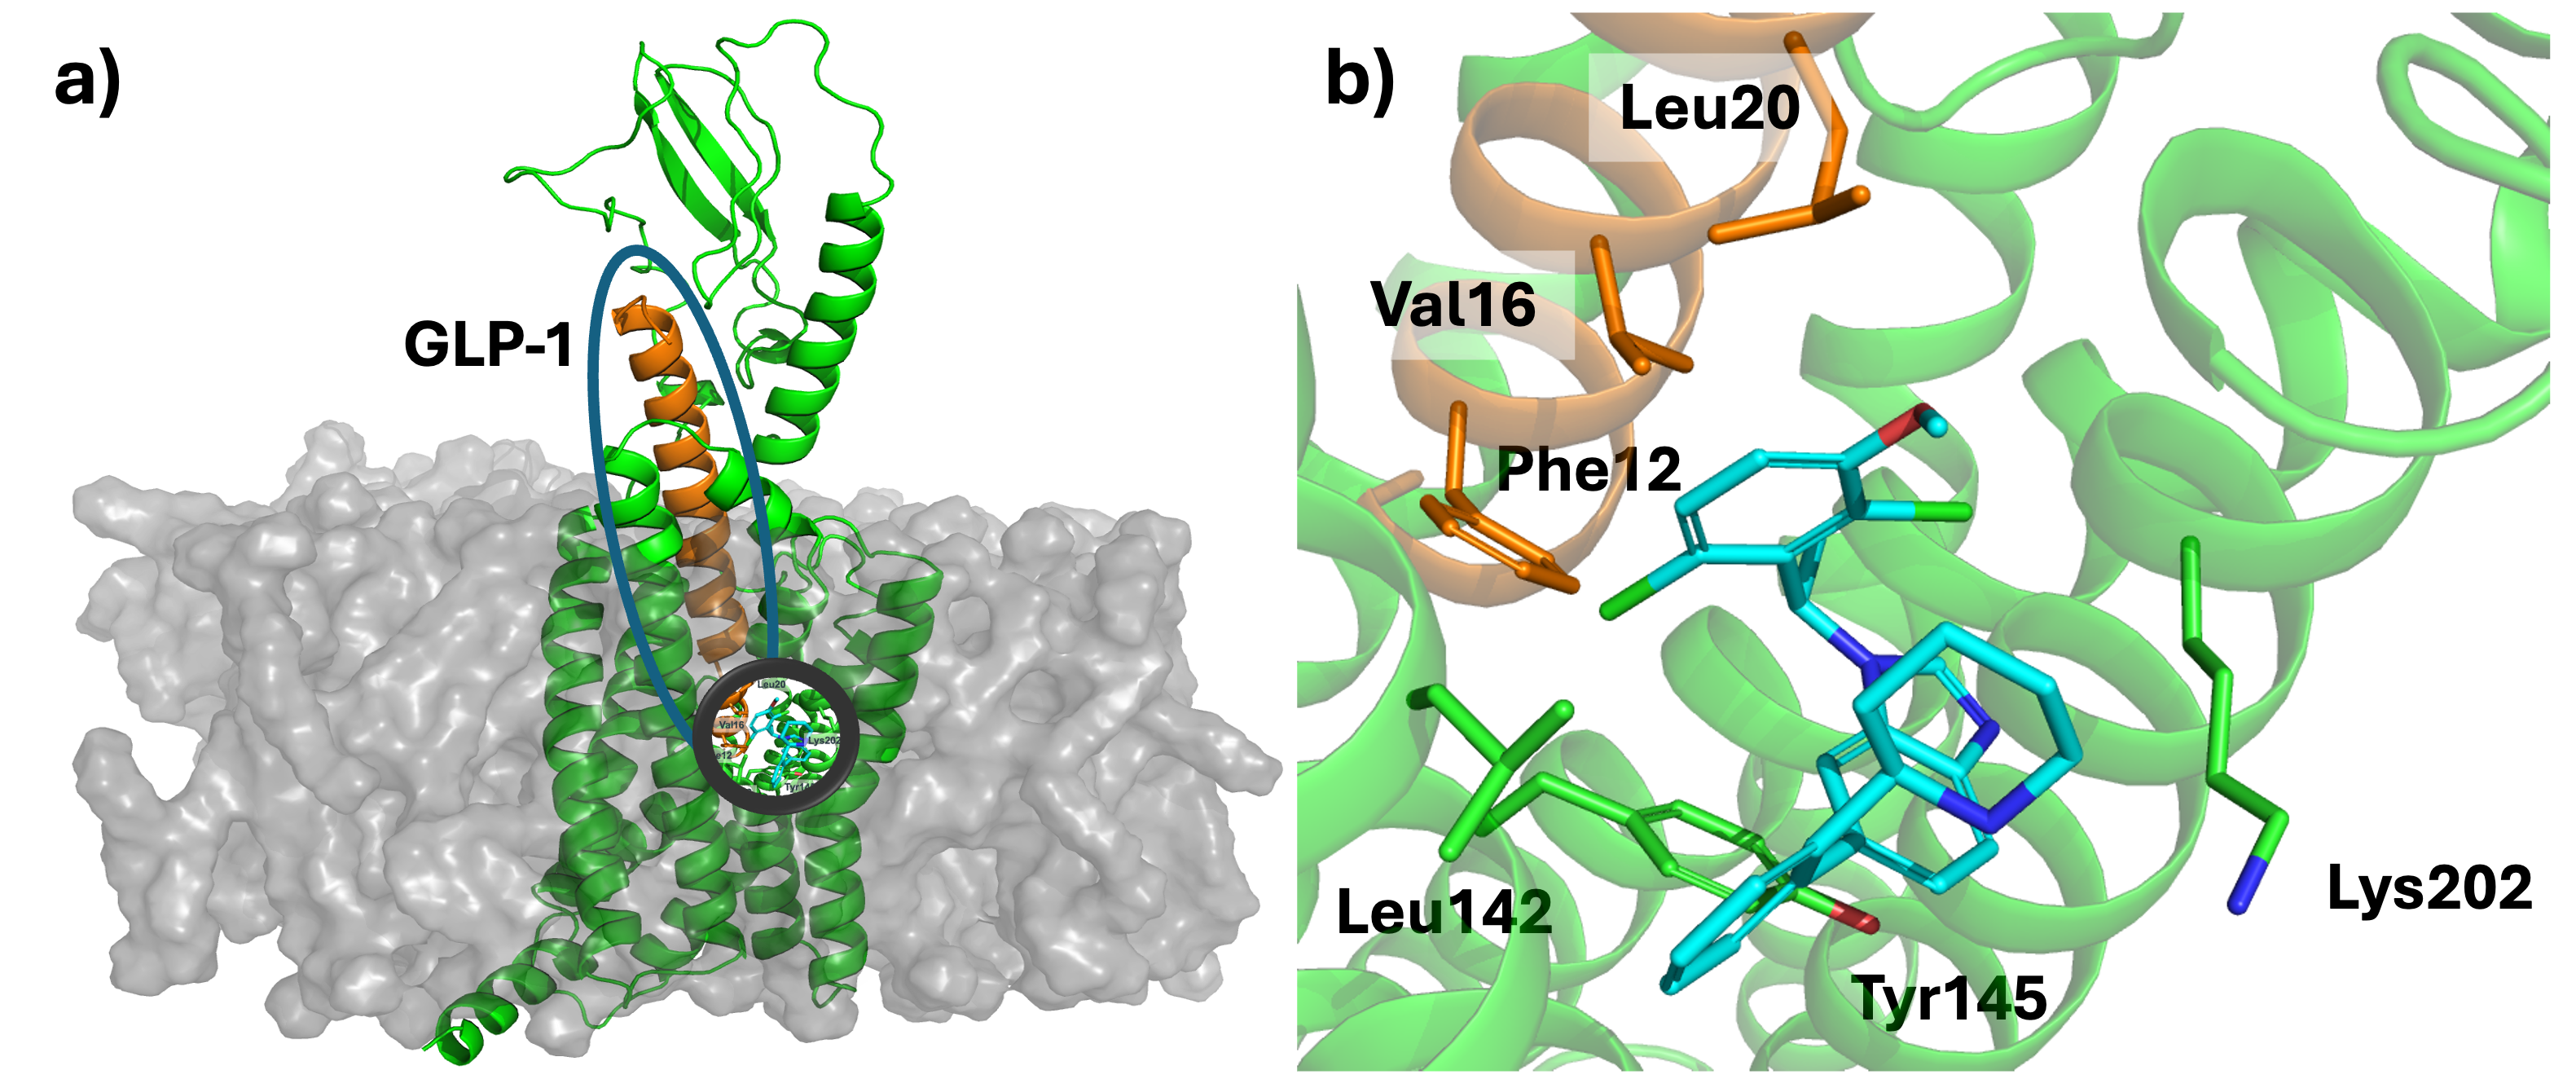
\includegraphics[width=0.5\textwidth]{Figures/lsn-interactions.png}
  \caption{\textbf{a)} Structure of GLP-1R (green) in complex with GLP-1 (orange), embedded in a POPC membrane, as used in MD simulations. GLP-1 is circled and depicted in orange. The binding site of compound LSN3160440 (PAM binding site) is highlighted. \textbf{b)} Binding mode of Compound LSN3160440 (ConformetRx) in the binding site highlighted in section \textit{a}. LSN3160440 acts as a molecular glue, stabilising the interactions between GLP-1 and GLP-1R through interactions with Phe12, Val16 and Leu20 (GLP-1) and Leu142, Tyr145 and Lys202 (GLP-1R).}
  \label{fig:lsn-interactions}
\end{figure}

\subsection{Exploration of the conformational space}\label{section:MD}

MD simulations of the \textit{apo} (GLP-1R + GLP-1) and \textit{holo} (GLP-1R + GLP-1 + LSN3160440) systems were performed to test the hypothesis that LSN3160440 acts as a molecular glue that enhances the affinity of the protein for its natural substrate, as well as to select snapshots to use later on in ensemble virtual screening. 

The structure of the GLP-1R+GLP+LSN3160440 complex was obtained from PDB entry 6VCB\cite{Bueno2020StructuralReceptor}, then embedded in a POPC bilayer using the CHARMM-GUI membrane builder\cite{Lee2016CHARMM-GUIField,Feng2023CHARMM-GUIApplications}. The system was placed the center of a rectangular box which extended as much as the membrane in the x and y directions, and 10 $\text{\AA}^{2}$ from the outer-most atom on each side in the z direction, then solvated in water. An \textit{apo} structure (GLP-1R + GLP-1) was generated by repeating the process and omitting the ligand. The force fields used in our MD simulations were the following: Amber99sb-ildn\cite{Lindorff-Larsen2010ImprovedField} for protein residues, GAFF2\cite{Wang2004DevelopmentField,TheFields} with AM1-BCC charges\cite{Jakalian2002FastValidation} for LSN3160440, Amber Lipid21\cite{Dickson2022Lipid21:AMBER} for the membrane and TIP3P\cite{Mark2001StructureK} for the water.

MD simulations were run using Gromacs 2023.3\cite{Abraham2015GROMACS:Supercomputers}. Both systems were minimised and equilibrated following the standard protocol implemented in CHARMM-GUI. A restrained minimisation was followed by two restrained NVT simulations of 125 ps each and using a 1 fs timestep. Subsequently, a restrained NPT simulation of 125 ns and 1 fs timestep was followed by three additional NPT stages of 500 ps at 2 fs timestep, during which the restraints were progressively released. Temperature and pressure (when enabled) were maintained at 303.15 K and 1 bar using the V-rescale thermostat\cite{Bussi2007CanonicalRescaling} and the C-rescale barostat\cite{Bernetti2020PressureRescaling}, respectively. Long-range electrostatics were treated using the Particle Mesh Ewald (PME) algorithm\cite{Darden1993ParticleSystems} and all bonds involving hydrogen were constrained using the LINCS algorithm\cite{Hess1998LINCS:Simulations}.

Once the systems were equilibrated, 4 unrestrained production replicates of 500 ns were run for each system using a time step of 2 fs and collecting snapshots every 100 ps. This amounted to a total of 8$\mu s$ of production simulations and 40000 snapshots.

The contact surface area between the ligand and the involved residues was calculated for all snapshots obtained form \textit{holo} simulations using the same methodology described in Section \ref{section:second_filter}. From those, the 10 snapshots with the highest values were identified as the ones displaying the strongest interactions between ligand and the relevant residues from GLP-1 and GLP-1R, and set aside for use in ensemble virtual screening.


\section{Results and Discussion}
\subsection{Selection of receptor structures}
The root mean square fluctuations (RMSF) of the residues of interest across all production snapshots of each system was calculated as a means to test the hypothesis that LSN3160440 acts as a molecular glue, stabilising the interaction between GLP-1R and GLP1. The values presented in Figure \ref{fig:rmsf} indicate that with the exception of Phe12 (GLP-1), all involved residues display lower RMSF in the \textit{holo} simulations. Of special interest is residue Lys202 (GLP-1R) which presents significantly lower fluctuations in the \textit{holo} simulations despite not interacting directly with the ligand in the crystal structure. This supports the hypothesis by Bueno \textit{et al.}\cite{Bueno2020StructuralReceptor} that this residue interacts with the ligand through a water-mediated hydrogen bond.

\begin{figure}[H]
\centering
  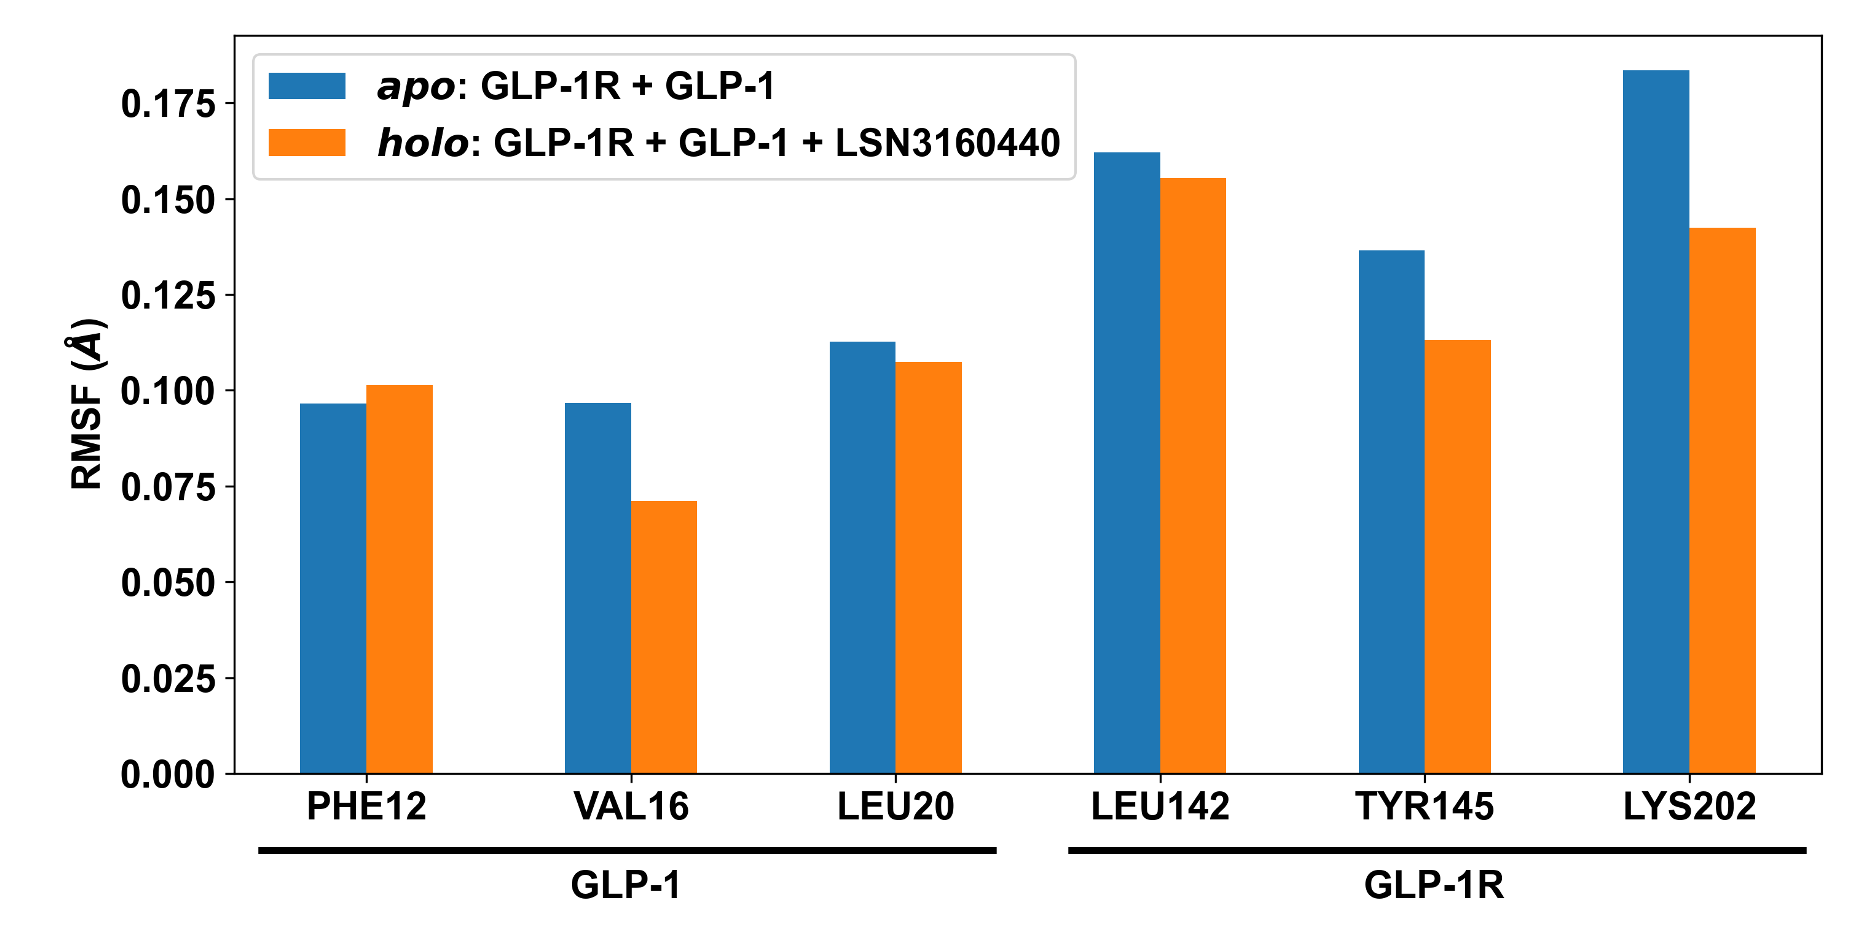
\includegraphics[width=0.5\textwidth]{Figures/rmsf.png}
  \caption{Comparison of the root mean square fluctuations of the residues from GLP-1R and GLP-1 involved in interactions with LSN3160440. Values obtained from aggregated MD trajectories of the \textit{apo} (blue) and the \textit{holo} (orange) systems. }
  \label{fig:rmsf}
\end{figure}

Figure \ref{fig:csa} presents the contact surface area between LSN3160440 and the residues of interest from GLP-1R and GLP-1 along each replicate of the \textit{holo} MD simulation. Since one of the goals of our workflow was to generate compounds with strong interactions with the same residues, the 10 snapshots with the highest CSA values were selected for the docking stage of our workflow.

\begin{figure}[H]
\centering
  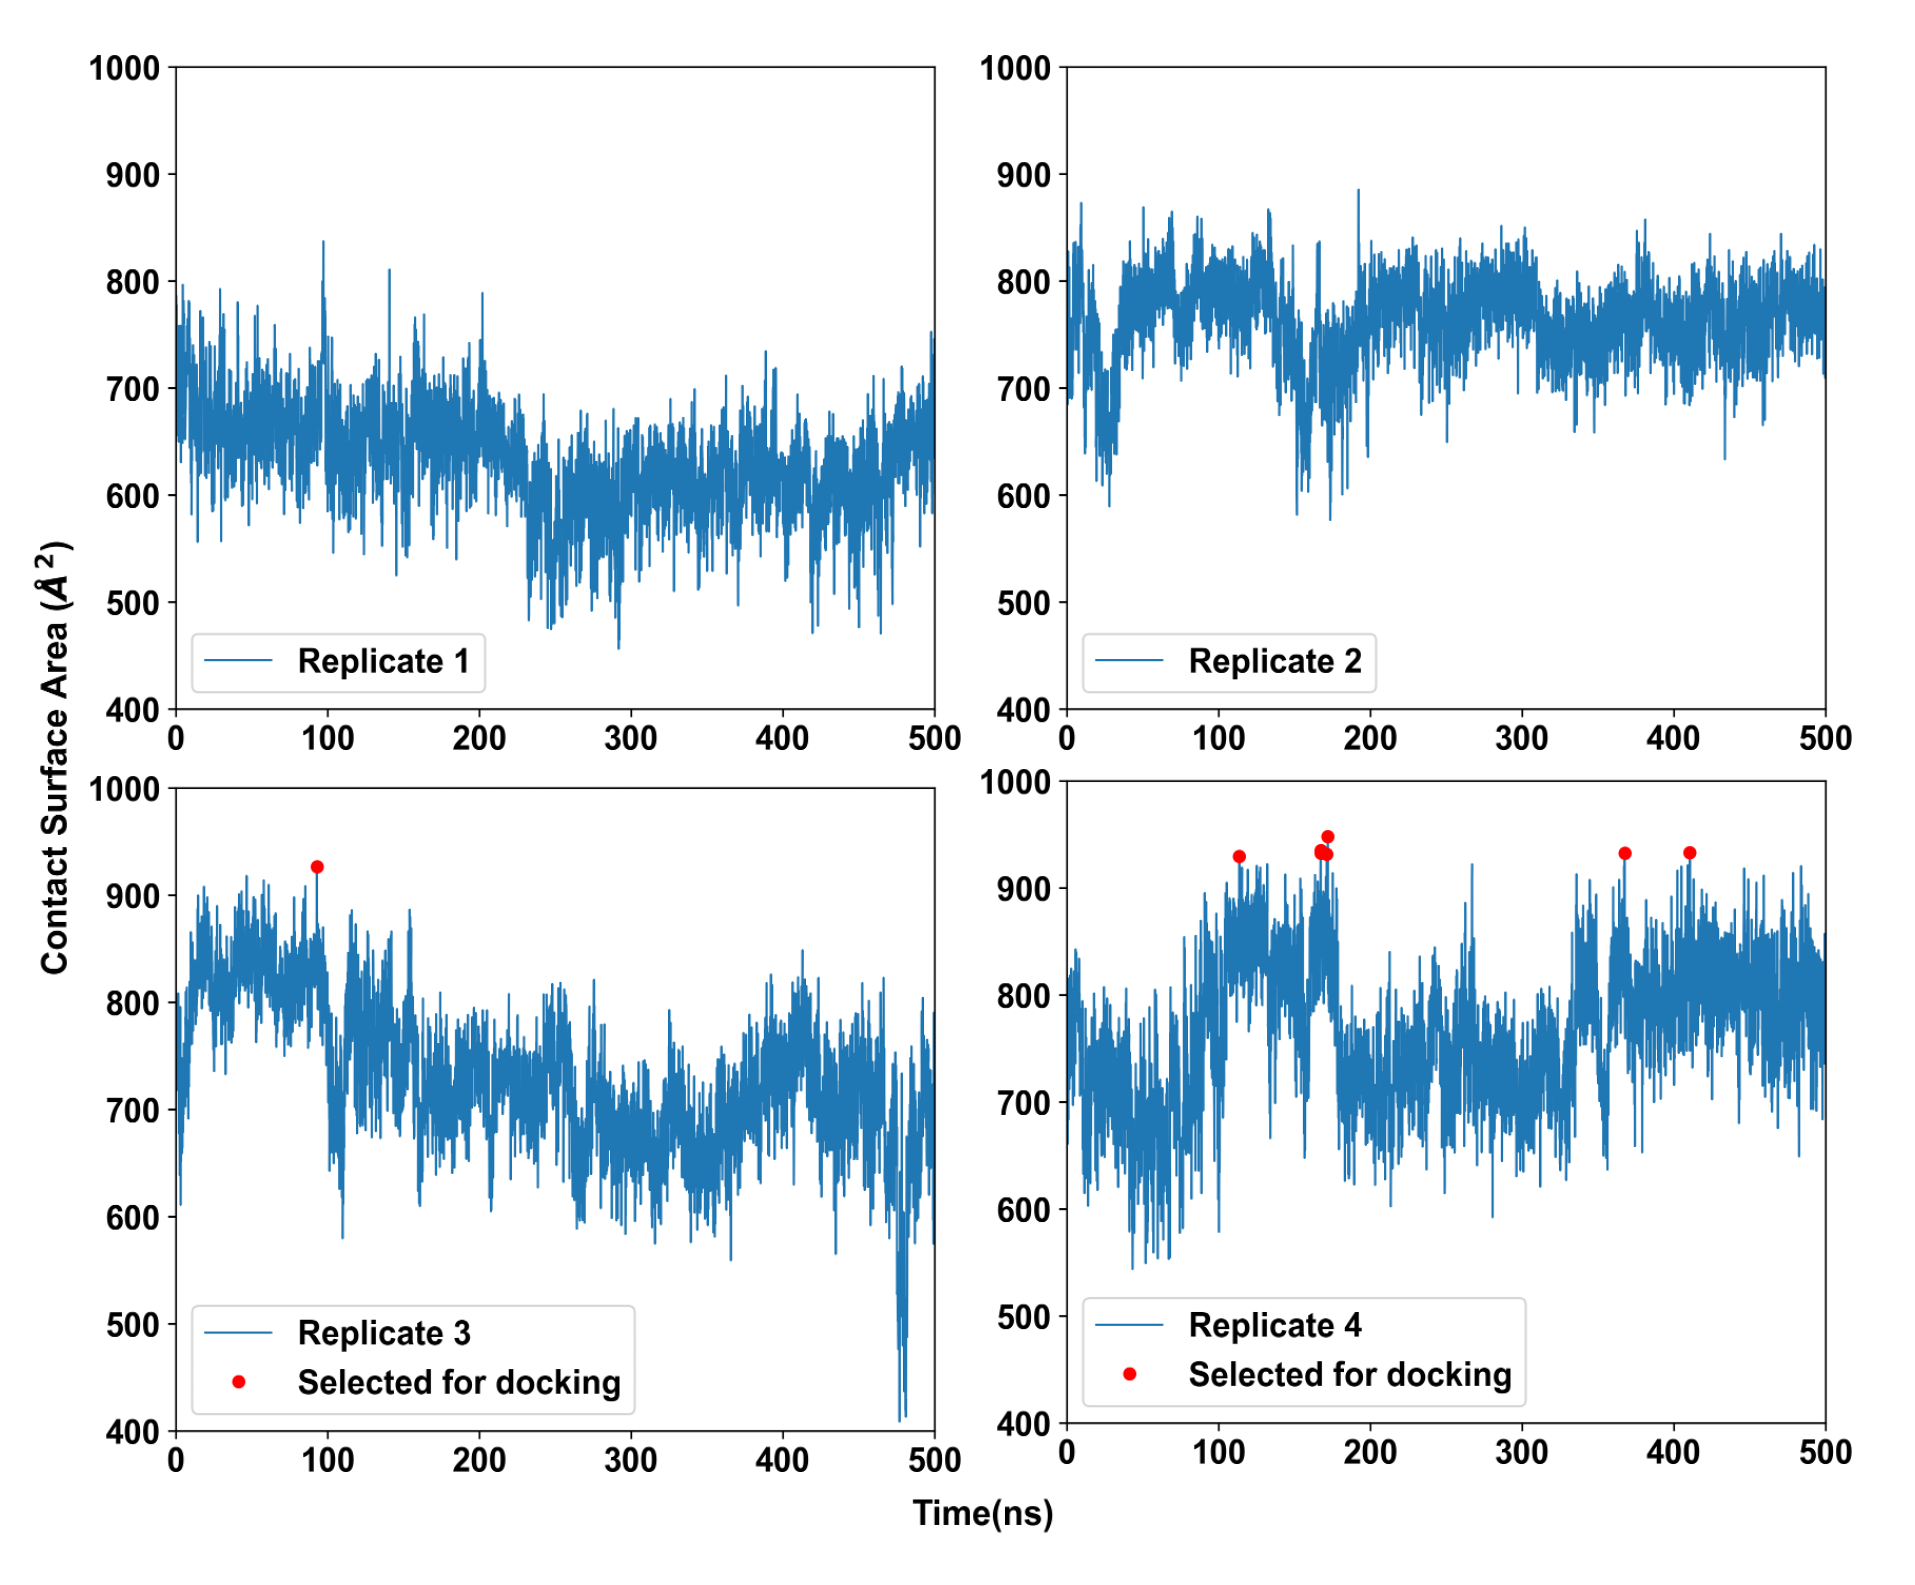
\includegraphics[width=0.5\textwidth]{Figures/CSA.png}
  \caption{Contact surface area between LSN3160440 and relevant interacting residues along each replicate of the \textit{holo} simulations. Snapshots highlighted with a red dot were selected for docking in the second filter of the Active Learning loop.}
  \label{fig:csa}
\end{figure}


\subsection{Evolution of Properties}
Figure \ref{fig:properties} presents the distributions of the values of the desired properties across all generated compounds that passed both filters at each iteration of the workflow. Overall, all properties except the Contact Surface Area show consistent improvement over the 5 iterations, demonstrating that our workflow is effective at generating molecules that increasingly match the desired properties. Additionally, the distributions of SA Score and QED extend beyond the values corresponding to LSN3160440 even for the first iteration of the workflow, highlighting the effectiveness of the Reinforcement Learning step at optimizing those properties. The effectiveness of the adaptive filtering strategy is evidenced by the consistent enrichment of the population in each iteration. 

\begin{figure}[H]
\centering
  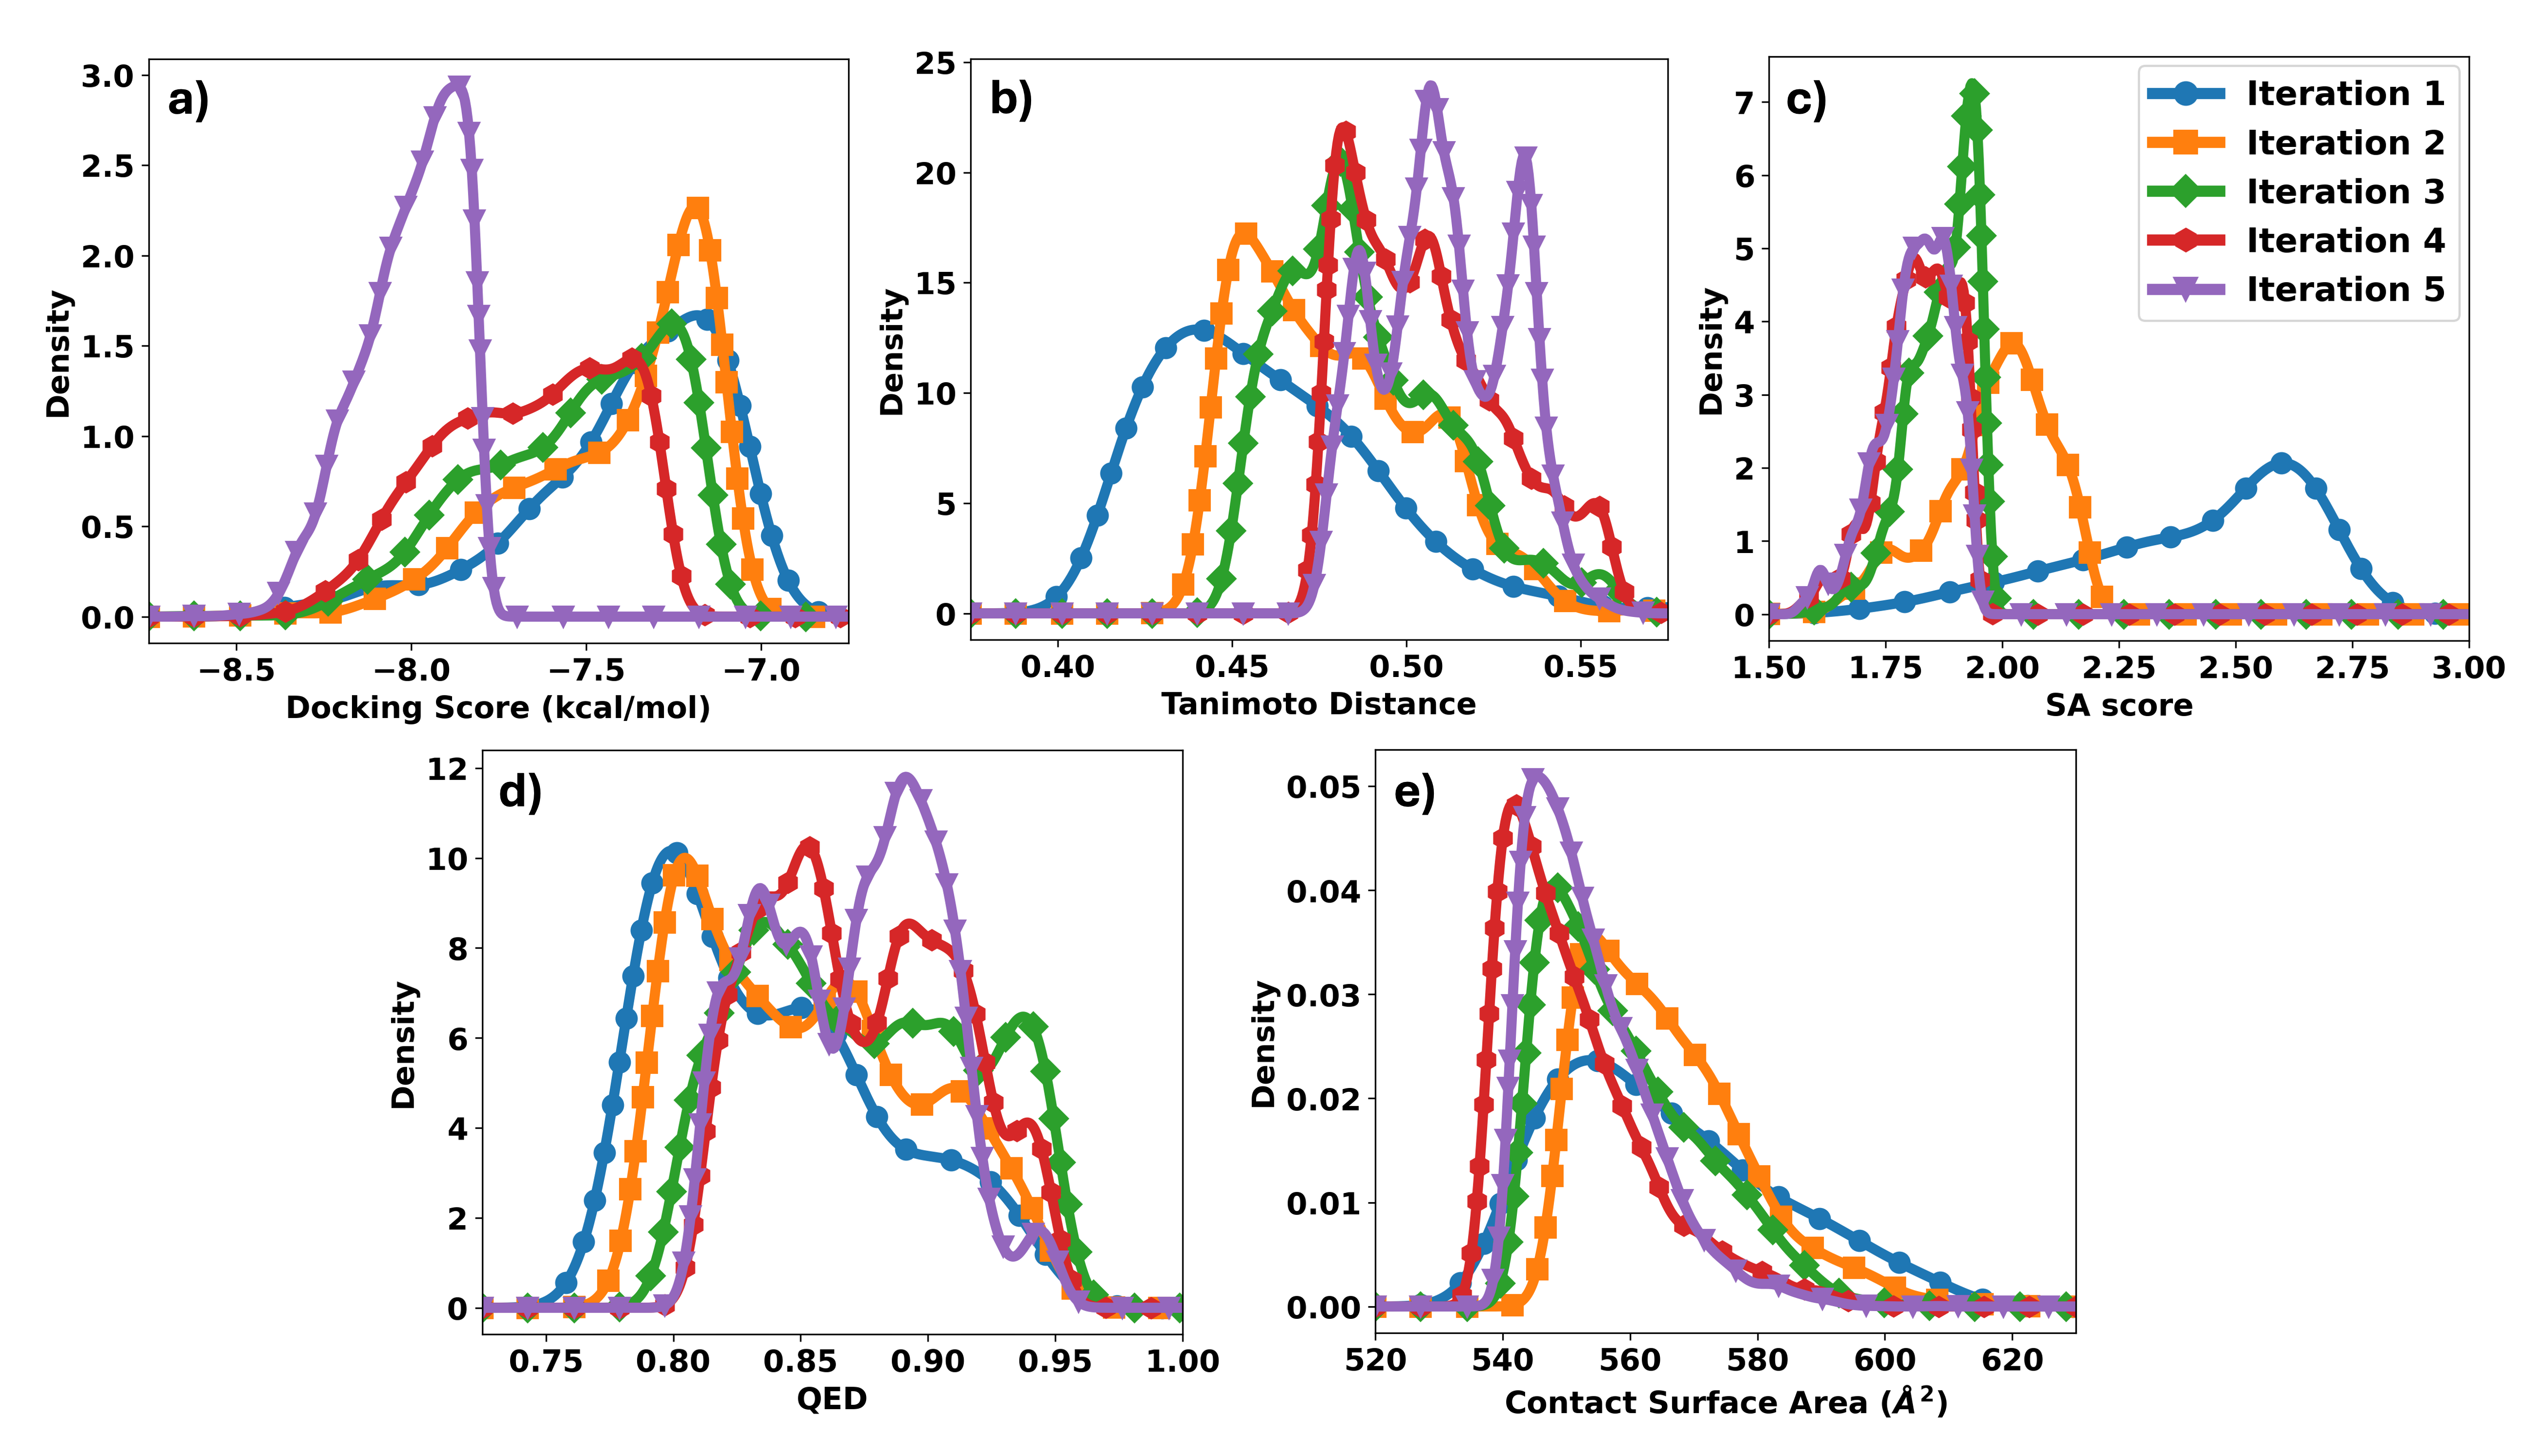
\includegraphics[width=\textwidth]{Figures/properties.png}
  \caption{Probability density distributions of the values of a) docking score, b) dissimilarity with the seed compound, c) synthetic accessibility, d) drug-likeness, and e) contact surface area between the docked compound and the residues of interest. The distributions corresponding to each iteration are indicated with colored lines and markers as follows: blue and circles for iteration 1, yellow and squares for iteration 2, green and diamonds for iteration 3, red and hexagons for iteration 4 , and purple and inverted triangles for iteration 5.}
  \label{fig:properties}
\end{figure}

Table \ref{tab:hist_bin_center} presents the values corresponding to the histogram peak at each iteration, for each of the properties of interest, in comparison with those calculated for compound LSN3160440, highlighting once more, that all properties except the CSA show a consistent improvement across iterations. Unlike fixed-threshold methods, which may stall if the generative model fails to produce molecules meeting an arbitrary cutoff, these iteration-specific thresholds ensure that the most promising subset of the current population is always leveraged for transfer learning.

\begin{table}[H]
  \caption{Value of the histogram bin with the maximum number of elements for each property at each iteration}
  \label{tab:hist_bin_center}
  \centering
  \begin{tabular}{cccccc}
    \hline
    Iteration            & Average       & Tanimoto & SA score & QED   & Average            \\
                         & Docking Score & Distance &          &       & CSA                \\
                         & (kcal/mol)    &          &          &       & ($\text{\AA}^{2}$) \\
    \hline
    1                    & -7.04         & 0.433    & 2.70     & 0.786 & 541                \\
    2                    & -7.10         & 0.447    & 2.15     & 0.806 & 549                \\
    3                    & -7.15         & 0.507    & 1.82     & 0.831 & 544                \\
    4                    & -7.27         & 0.507    & 1.82     & 0.813 & 538                \\
    5                    & -7.81         & 0.506    & 1.79     & 0.837 & 541                \\
    \hline
    LSN3160440                  & -7.95         & --       & 4.06     & 0.357 & 560                \\
    \hline
  \end{tabular}
\end{table}

\subsubsection{Docking Score}\label{sec:results-docking_score}
The docking score, as calculated by Vina-GPU, is an estimation of the binding energy between the receptor and the ligand, expressed in kcal/mol. As such, the lower the value of the docking score, the stronger the interaction between the receptor and the ligand is estimated to be. Figure \ref{fig:properties}A, presents the evolution of the average docking score (among the 10 selected MD snapshots) across the 5 iterations of our workflow, displaying a consistent improvement of that property at each iteration. It is also noteworthy that the amount of compounds that exhibit an average docking score better than that of LSN3160440 also improves consistently.

\subsubsection{Dissimilarity with seed compound (Tanimoto Distance)}
The dissimilarity of the generated molecules to LSN3160440 was expressed in terms of their Tanimoto Distance, calculated using Morgan fingerprints\cite{Raymond2002EffectivenessDatabases}. Figure \ref{fig:properties}B shows that the molecules generated at each iteration of the workflow increasingly differ from LSN3160440. As the number of iterations increases, it can be seen that the corresponding distributions present multiple peaks, however, for a given distribution, even the lowest peak is always at a higher value than the higest peak of the previous iteration.

\subsubsection{Synthetic Accessibility Score (SAScore)}
The synthetic accessibility of the generated molecules is expressed in terms of RDKit's SA Score\cite{Ertl2009EstimationContributions}. This is a rules-based method based on a combination of fragment contributions and a complexity penalty, which results in a value ranging from 1 (easily synthesizable) to 10 (very difficult to synthesize). Figure \ref{fig:properties}C shows the evolution of the SA score along the 5 iterations of the workflow. After the first iteration, where the distribution is centered at 2.70, the distribution of the SA score quickly improves, and converges at values around 1.8, indicating that the molecules generated by the workflow are reaching a maximum synthetic accessibility.

\subsubsection{Quantitative Estimation of Drug-likeness (QED)}
The concept of QED was originally introduced by Bickerton and coworkers\cite{Bickerton2012QuantifyingDrugs,Wildman1999PredictionContributions}, taking into account the distribution of properties such as molecular weight, $logP$, hydrogen-bond donors and acceptors, aromatic rings, and unwanted moieties, among others. The RDkit implementation of QED produces a descriptor with values ranging from 0 (not drug-like) to 1 (maximum drug-likeness). Figure \ref{fig:properties}D presents distributions where the maximum shifts consistently towards 1, but with a high degree of overlap. This indicates that while this property does improve at each iteration of the workflow, REINVENT4 already produces molecules with high predicted oral bioavailability, leaving little room for improvement. 

\subsubsection{Contact Surface Area}
The Contact Surface Area (CSA) between the generated molecules and the relevant residues from GLP-1R and GLP-1 is the only descriptor that does not show a consistent improvement along the 5 iterations of the workflow, but rather a set of distributions with a high degree of overlap and the peaks of which do not seem to show any specific shift. The average value of the CSA between the residues of interest and compound LSN3160440, among the snapshots selected for docking, is 673 $\text{\AA}^{2}$, while the distributions of the generated molecules all peak at approximately 550 $\text{\AA}^{2}$. We suspect that this is mainly due to the inability of our workflow to take into account water-mediated interactions such as that between residue Lys202 of GLP-1R and LSN3160440, opening up an avenue for improvement, and, as discussed in Section \ref{sec:results-mw}, the smaller size of the generated molecules.

\subsubsection{Molecular weight and binding efficiency}\label{sec:results-mw}
The last iteration of the workflow produced a library of 5370 compounds. Among those, 4834 outperformed compound LSN3160440 in terms of average docking score, while 4984 outperformed it in terms of best docking score. Additionally, all 5370 compounds retained after iteration 5 have lower molecular weight than LSN3160440, suggesting that our workflow generates compounds with a higher binding efficiency than the chemical starting point, even though the molecular weight of the generated molecules was not taken into account at any stage of the process. 

To test this hypothesis, the binding efficiency of a compound can be expressed as its docking score (best or average) divided by its molecular weight. To obtain a reference point, we calculated the binding efficiency of compound LSN3160440 in the same way, leading to the calculation of the Relative Binding Efficiency (RBE) parameter using Equation \ref{eq:RBE}

\begin{equation}
\label{eq:RBE}
    RBE=\frac{Score_{cpd}/MW_{cpd}}{Score_{LSN}/MW_{LSN}}
\end{equation}
where $Score$ refers to the docking score of a given compound, $MW$ refers to its molecular weight, and the subscripts $cpd$ and $LSN$ indicate the compound of interest and LSN3160440, respectively.

Figure \ref{fig:beff} presents the distributions of molecular weights and RBE values of the compounds that passed both filters at each iteration of the workflow. As the workflow advances, the model tends to generate molecules with lower molecular weight and, as presented in Section \ref{sec:results-docking_score}, better docking scores, resulting in the fact that the RBE with respect to LSN3160440 consistently increases as more iterations are run. An unexpected result is that the retained compounds generally exhibit a higher binding efficiency than LSN3160440, even during the first iterations of the workflow, highlighting the capability of the REINVENT4 prior to generate high quality molecules even before fine-tuning.

Additionally, lower molecular weights suggest that the generated molecules have a lower SASA. This can lead to a lower contact surface area between the ligand and the residues of interest, explaining why this is the only property that did not consistently improve as we ran more iterations of our workflow.

\begin{figure}[H]
\centering
  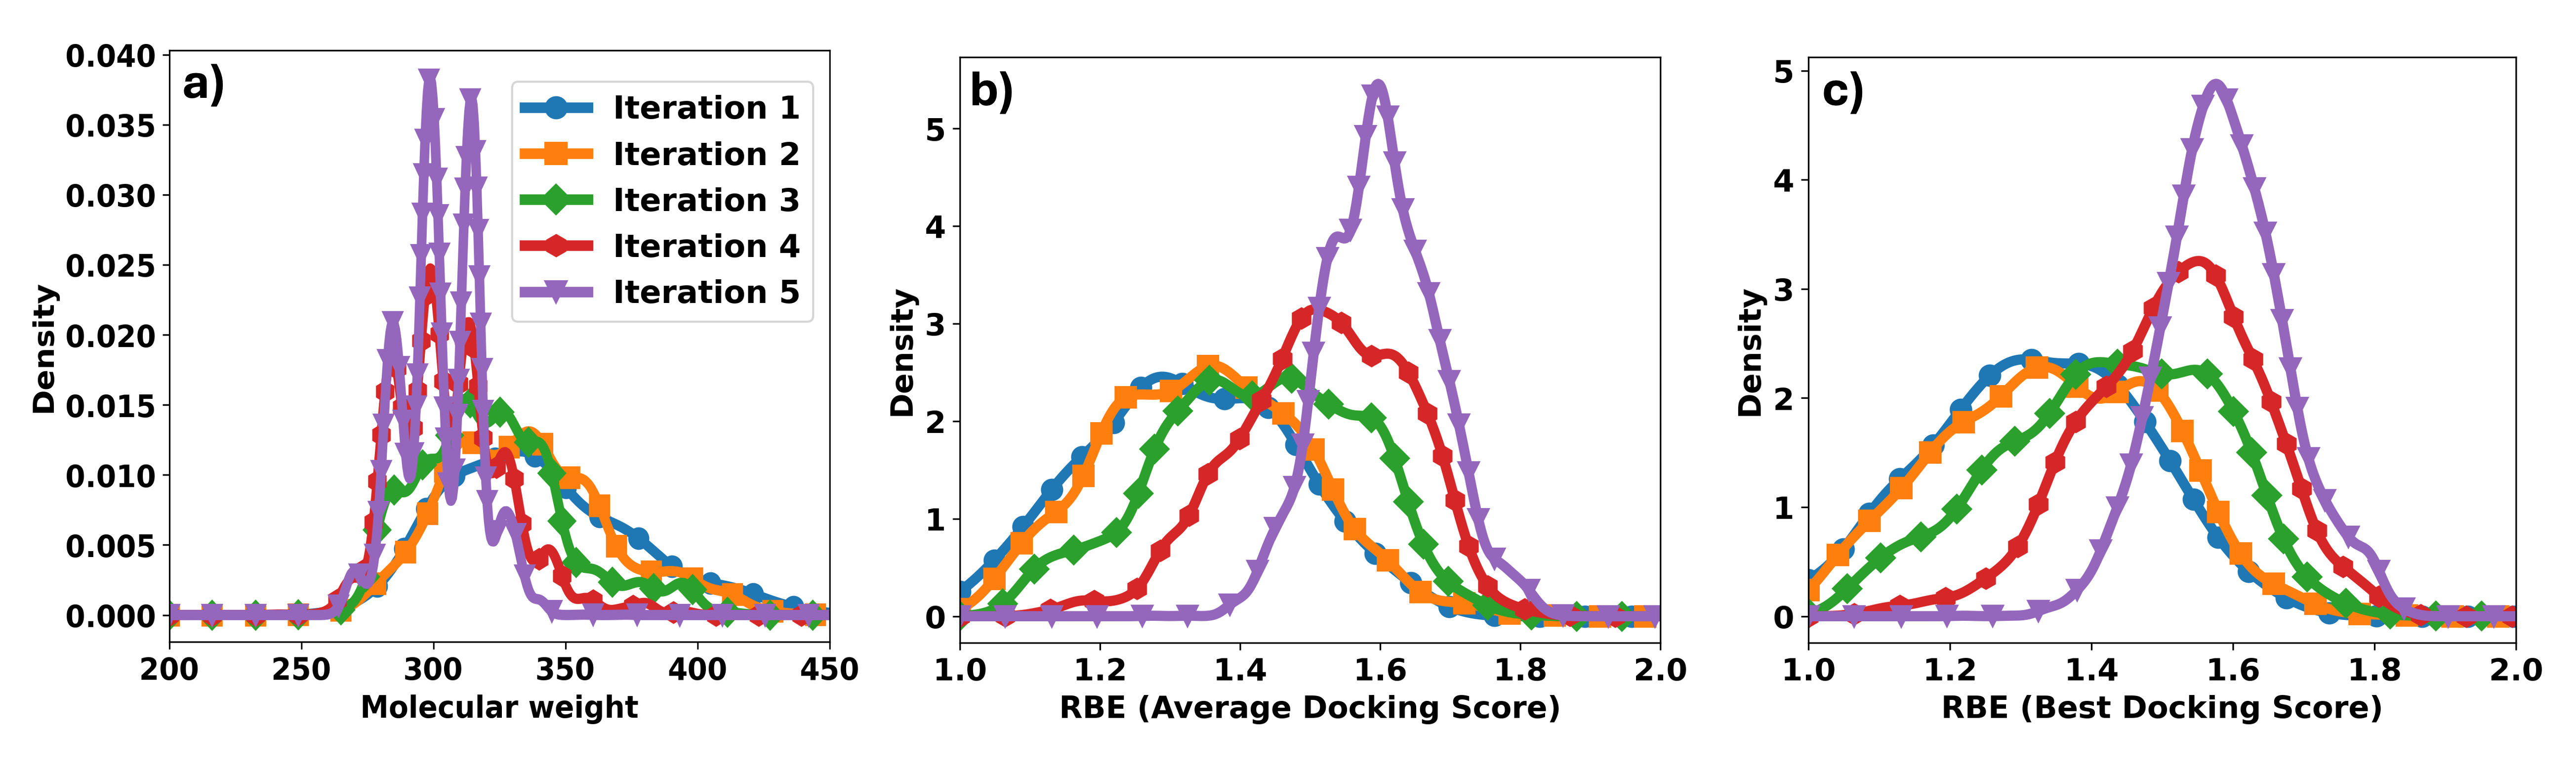
\includegraphics[width=\textwidth]{Figures/beff.png}
  \caption{Probability density distributions of the values of a) Molecular weight of the generated molecules; b) Relative Binding Efficiency (RBE) with respect to compound LSN3160440, calculated using the average docking score of each compound; c) RBE, calculated using the best docking score of each compound. Distributions are calculated only for the compounds that passed both filters at each iteration. The distributions corresponding to each iteration are indicated using the same colour scheme as in Figure 4.}
  \label{fig:beff}
\end{figure}


\subsection{Library enrichment and diversity}
Table \ref{tab:library_enrichment} presents the number of compounds that were generated and those that progressed through each filter, along the 5 iterations of our protocol, as well as a measure of the diversity of the final dataset obtained after each iteration (the compounds that progressed to TL). For consistency, the dataset diversity was expressed as the average pairwise Tanimoto distance of each dataset, calculated using the same fingerprints and parameters as in its REINVENT4 implementation.  
\begin{table}[H]
  \caption{Number of compounds present at each stage of the active learning loop, across 5 iterations of the protocol}
  \label{tab:library_enrichment}
  \centering
  \begin{tabular}{ccccc}
    \hline
    Iteration & Compounds & Compounds & Compounds   & Average\\
              & generated & progressed & progressed & diversity\\
              & by RL     & to VS      & to TL\\
    \hline
    1 & 125985 & 1134  & 286  & 0.8484\\
    2 & 169741 & 9009  & 1568 & 0.7813\\
    3 & 116437 & 13404 & 3422 & 0.7292\\
    4 & 118060 & 19359 & 5634 & 0.7090\\
    5 & 116855 & 29134 & 5370 & 0.6579\\
    \hline
  \end{tabular}
\end{table}
Across 5 iterations of our active learning cycle, we observed that the number of compounds that passed both filtering steps consistently increases, highlighting the effectiveness of the workflow at improving the generated models.The number of compounds that progress to the Virtual Screening Stage increases by approximately 30 times between iterations 1 and 5, while the number of compounds that are selected for Transfer Learning increases approximately 25-fold, indicating that both filters are approximately equally effective.
An unexpected consequence of the workflow is the consistent decrease in the diversity of the datasets. This observed decrease in diversity highlights a classic 'exploration-exploitation' trade-off inherent in multi-objective RL workflows. The convergence toward specific regions of chemical space likely reflects the model’s adaptation to the 10 specific receptor conformations used in the ensemble docking filter. To mitigate this in future studies, the diversity filter penalties could be dynamically weighted, or the receptor ensemble could be expanded to include a broader range of metastable states identified via MD 

\subsection{Binding modes of selected compounds}

The two compounds with the best average docking scores, namely 5.4870 and 5.24889 were selected for further investigation. Figure \ref{fig:new_molecules} presents the conformations of GLP-1R and GLP-1 bound to these compounds. The interactions between those compounds and the GLP-1R/GLP-1 system are essentially the same as those with compound LSN3160440, a consequence of repeatedly fine-tuning the model with the compounds that showed the highest contact surface area with the residues that are relevant for the glue effect of LSN3160440. It is worth noting that Autodock Vina (underlying algorithm of Vina-GPU) does not account for water-mediated hydrogen bonds such as the one between LSN3160440 and residue Lys202. None of the molecules selected for further investigation presents a direct hydrogen-bond with Lys202, suggesting that this residue can only interact with the binding site through water molecules. Therefore, we speculate that with the use of a docking tool that includes structural water molecules, our workflow would produce molecules with even stronger interactions.

\begin{figure}[H]
\centering
  \includegraphics[width=0.5\textwidth]{Figures/new_molecules.png}
  \caption{Binding modes of Compounds a) LSN3160440 and b) 5.4870 and c) 5.24489. The structure of the GLP-1R/GLP-1 system that binds LSN3160440 is included in sections \textit{b} and \textit{c}, with transparent cartoon and thin lines for the relevant residues, as a means of comparison. d) 2D structures of the compounds presented in sections \textit{a}, \textit{b}, and \textit{c}.}
  \label{fig:new_molecules}
\end{figure}

Table \ref{tab:new_molecules} presents the values of the calculated physico-chemical descriptors of Compounds 5.4870 and 5.24489, along with those of LSN3160440, highlighting the improvement on all properties with the commented exception of the Contact Surface Area. Additionally, the Tanimoto distance between these 2 compounds, 0.641, is comparable to that between each of them and LSN3160440. This suggests that, although the diversity of the molecules decreases with the number of iterations, the workflow is still capable to produce molecules that substantially differ from each other.

\begin{table}[H]
  \caption{Descriptor values of compounds selected for further investigation, in comparison with LSN3160440.}
  \label{tab:new_molecules}
  \centering
  \begin{tabular}{cccc}
    \hline
    Property & LSN3160440 & Compound & Compound \\
             &     & 5.4870   & 5.24889 \\
    \hline
    Average Docking Score & -7.95 & -8.57 & -8.63\\
    (kcal/mol) & & & \\
    Best Docking Score & -9.0 & -9.5 & -9.1\\
    (kcal/mol) & & & \\
    Tanimoto Distance & -- & 0.500 & 0.528\\
    \textit{w.r.t} LSN3160440 & & & \\
    SA score & 4.06 & 1.844 & 1.818\\
    QED & 0.357 & 0.842 & 0.828\\
    Average CSA ($\text{\AA}^{2}$) & 673 & 573 & 560\\
    Highest CSA ($\text{\AA}^{2}$) & 713 & 618 & 619\\
    Molecular weight (g/mol) & 480 & 325 & 311\\
    \hline
  \end{tabular}
\end{table}

\section*{Conclusions}
In this work, we have presented a workflow that combines the Reinforcement Learning and Transfer Learning capabilities of REINVENT4 with structure-based methods such as ensemble Virtual Screening and Contact Surface Area calculations, in order to strengthen the ability of the generative model to produce molecules that increasingly match the desired set of properties. The main innovative characteristic of our workflow is the fact that a generated compound only progresses to the next round if its scores for all properties taken into account surpass the value corresponding to the peak of their respective distributions. This workflow is model- and property- agnostic in principle: it can be implemented using any generative framework with Reinforcement Learning and Transfer Learning capabilities, as well as any property of interest. Additionally, adding a filter based on the negative-log likelihood of the generated molecules ensures that only molecules that are less likely to be sampled (the \textit{edges} of the model) are used to refine the model for further iterations, increasing the probability of generating novel molecules.

As a test case, we have applied this model to the generation of Positive Allosteric Modulators of GLP-1R, and we have demonstrated that most of the properties taken into account consistently improve and that better and larger datasets are produced. We have also identified limitations of our workflow such as its inability to account for water-mediated interactions between the receptor and the ligand, and the decrease of dataset diversity at eacgh iteration, which we have hypothesized is due to the choice of receptor conformations at the docking stage. Those limitations provide room for improvement and are currently under investigation.

Overall, our work provides the community with an innovative workflow that can help address the lack of chemical matter for certain targets, having a potential impact in drug discovery and model development.


\section*{CRediT authorship contribution statement}
\textbf{J.C.N.}: conceptualisation, methodology, investigation, software, formal analysis, visualisation, writing (original draft), writing (reviewing and editing), project administration.
\textbf{A.P.}: conceptualisation, formal analysis, Visualisation, writing (reviewing and editing), supervision, project administration.
\textbf{A.M.}: formal analysis, visualisation, writing (reviewing and editing).

\section*{Conflicts of interest}
The authors declare that they have no known competing financial interests or personal relationships that could have appeared to influence the work reported in this paper. 

\section*{Data availability}
The following supplementary information is attached to this manuscript:
\begin{itemize}
    \item RL and TL input files used in REINVENT4.
    \item Reinvent prior used.
    \item CSV files with the compounds that passed the first filter at each iteration of the workflow. Contains RDkit descriptors, docking scores and CSA values.
    \item PDB files of the receptor conformations used for docking.
\end{itemize}
In addition, the python and bash scripts used in this work can be checked at \textit{https://github.com/carajillu/genai}. However, we are still on the process of putting them together in a ready-to-download tool.

\section*{Acknowledgements}
J.C.N. was funded by the Engineering and Physical Sciences Research Council (EPSRC) grant "CP2K For Emerging Architectures and Machine Learning", and they would like to thank EPSRC (Grant Ref. EP/W030489/1) and Matt Watkins (grant principal investigator) for the funding that enabled them to contribute to this work. 

%%%END OF MAIN TEXT%%%

%The \balance command can be used to balance the columns on the final page if desired. It should be placed anywhere within the first column of the last page.

\balance

%If notes are included in your references you can change the title from 'References' to 'Notes and references' using the following command:
%\renewcommand\refname{Notes and references}

%%%REFERENCES%%%
\bibliography{references_mendeley}
\bibliographystyle{rsc} %the RSC's .bst file

\end{document}
